\section{Постановка проблеми}
 
Системами голосового управління автомобілів забезпечується управління їх деякими функціями на основі і з використанням голосових команд. Ці команди зазнають перетворень в керуючі сигнали з наступною передачею їх відповідальним за це системам автомобіля. Системи голосового управління напрямлені на те, щоб водії не відволікалися під час практичного керування автомобілем для наступного досягнення комфорту і безпеки руху. Власними назвами володіють ряд систем голосового управління, якими є: Linguatronic від Mercedes-Benz, Ford Sync, Cadillac User Experience \cite{art1,Kravchenko_2009,Heisterkamp_2001,Jonsson_2009}. На марках автомобілів Audi, BMW, Kia, Lexus установлені системи голосового управління для зручності і забезпечення комфорту водіїв. Для систем голосового управління характерна різниця, що полягає у кількості підтримуваних мов, належному рівню при розпізнаванні команд, числі реалізації функцій управління. Найбільшою кількістю мов (19) володіє система «Ford Sync», крім того арсенал включає і російську мову, але української – немає. Значною роллю при управлінні дистрибуцією відрізняються процеси голосової взаємодії, в яких відбувається автоматизація з метою підвищення ефективності, збереження ресурсів тощо. Саме модель голосової взаємодії водія в системах диспетчерського контролю потребує автоматизації для підвищення ефективності процесу дистрибуції.

\section{Аналіз останніх досліджень і публікацій}

Системи голосового управління істотно різняться за рівнем розпізнавання команд. Відходять у минуле системи, в яких голосові команди для кращого розпізнавання проговорюються по буквах, що дуже незручно при використанні. Сучасні системи голосового управління успішно справляються з розмовною мовою, різними діалектами, альтернативними формулюваннями, індивідуальними особливостями вимови і швидкістю мови. Для підвищення якості розпізнавання команд використовується фільтр шумів, що відтинає непотрібні звуки.

Стандартними функціями, реалізованими за допомогою системи голосового управління, наприклад, компаніями Ford Motor Company, BMW AG, Daimler AG, є управління телефоном, мультимедійною системою, навігаційною системою, системою клімат-контролю \cite{Kravchenko_2009,Heisterkamp_2001,Jonsson_2009}.

Слід зазначити, що для випадку наявності достатньо потужної системи, голосову взаємодію з водієм можна використовувати для підтримання діалогу під час руху вночі, аби не дати водію заснути \cite{Kravchenko_2012}.
Також проводилися дослідження з розробки систем мовного управління бортовим обладнанням літаків, але через високі вимоги до швидкості та якості розпізнання, особливо за наявності потужних шумів та перешкод, вони ще досі не були запроваджені \cite{Korsun_2013}.

Використання таких часткових функцій голосового управління, які підвищують комфорт водія, також повинно мати певний позитивний ефект. Проте ці функції не забезпечують оптимізації саме процесів дистрибуції.


\section{Постановка завдання}

У даній статті необхідно запропонувати та розробити модель голосової взаємодії водія в системах диспетчерського контролю за рухом автотранспорту.

\section{Виклад основного матеріалу}

Підхід, який існує для голосового управління, заснований на теорії несилової взаємодії \cite{Teslia_2010} – рефлекторна система голосового управління \cite{Egorchenkov_2016,Teslia_2013}. Ідея, покладена в основу цього підходу, полягає в тому, щоб замість переведення голосової інформації в текстову репрезентацію, аналізувати безпосередньо інформаційну складову сказаного, визначаючи, яку з відомих реакцій потрібно виконати. «Традиційні системи розпізнання мови засновані на принципі: „усна мова“ → „репрезентація мови набором лінгвістичних конструкцій“ → „розуміння мови“. На основі теорії несилової взаємодій може бути запропонована інша модель розпізнання природної мови: „усна мова“ → „розрахунок несилової (інформаційної) взаємодії на реакції“ → „реакція (розуміння чи поведінка)“» \cite{Teslia_2014}.

Така модель розпізнання називається рефлекторною, оскільки побудована за аналогією зі структурою умовного рефлексу, в якому виділяються афектори, центральний компонент та ефектори. Така модель може бути добре поєднана з ідеєю використання дерева сценаріїв, оскільки сценарії також складаються із реакцій, і одиницею моделювання стає не лінгвістична особливість мовлення, а реакція (або команда), яка може бути врахована автоматизованою системою підрахунку маршрутів.

Використовуючи рефлекторну модель, здійснимо моделювання взаємодії між диспетчером та водієм на етапі дистрибуції «склад – точка доставки», тобто доставку продукції від складу до дверей клієнта, наприклад, для кур’єрських служб, що пов’язані з доставкою замовлень Інтернет-магазинів або доставкою бутильованої води тощо.

Для вищенаведеного у роботі приведена розробка дерева сценаріїв, яке може бути застосоване для голосової взаємодії суб’єктів дистрибуції «склад – дорога – точка доставки». Найпростіше дерево сценаріїв для моделі голосової взаємодії водія в системах диспетчерського контролю за рухом автотранспорту можна представити наступним чином (рис. \ref{img:01_simplest_positive_scenario}).

Найпростіше дерево сценаріїв (рис. \ref{img:01_simplest_positive_scenario}) показує всі доступні варіанти (послідовність подій) у моделі голосової взаємодії водія в системах диспетчерського контролю за рухом автотранспорту. Кожна така послідовність або ланцюжок подій повинен представлятися окремим сценарієм.

\begin{figure}
	\centering
	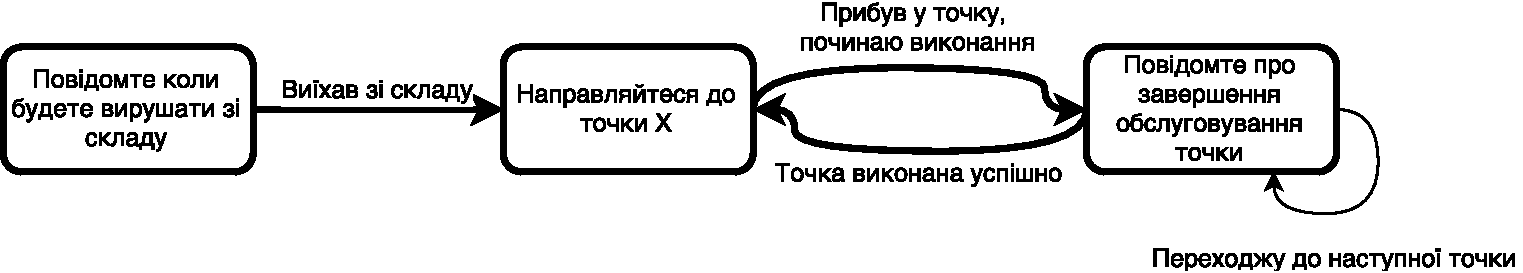
\includegraphics [width=.8\linewidth] {01_simplest_positive_scenario}
	\caption{Найпростіше дерево сценаріїв}
	\label{img:01_simplest_positive_scenario}
\end{figure}

Для випадку позитивного підтвердження обслуговування або виконання відповідної точки у моделі голосової взаємодії водія в системах диспетчерського контролю за рухом автотранспорту побудовано позитивне дерево сценаріїв (рис. \ref{img:03_positive_scenario_with_conformation}).

\begin{figure}
	\centering
	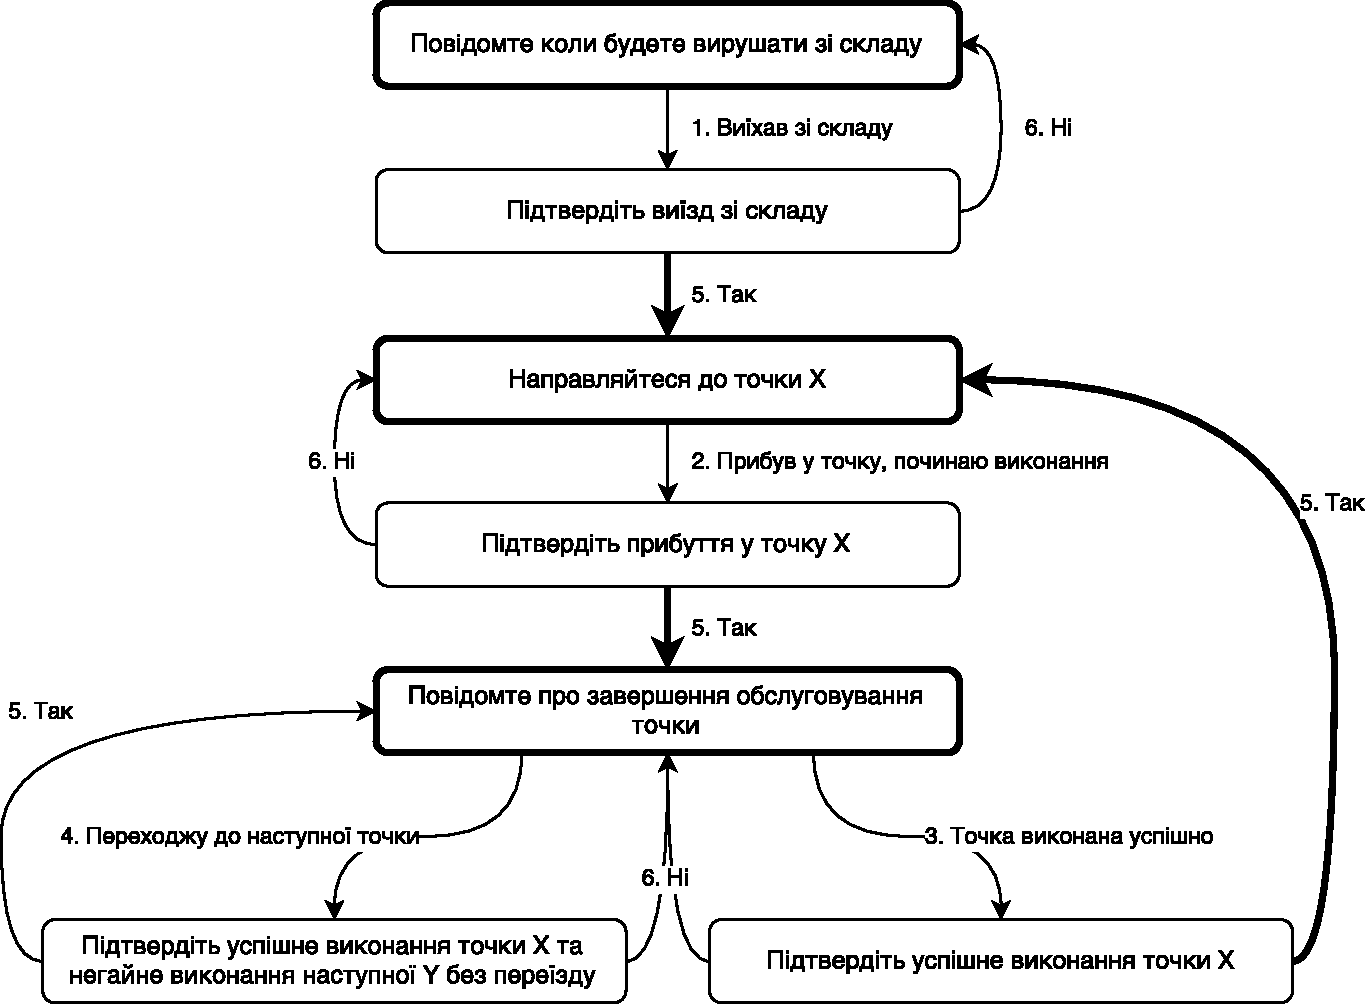
\includegraphics [width=.8\linewidth] {03_positive_scenario_with_conformation}
	\caption{Позитивне дерево сценаріїв з підтвердженням}
	\label{img:03_positive_scenario_with_conformation}
\end{figure}

Наведене позитивне дерево сценаріїв з підтвердженням обслуговування або виконання відповідної точки (рис. \ref{img:03_positive_scenario_with_conformation}) є більш складним у порівнянні з найпростішим деревом сценаріїв (рис. \ref{img:01_simplest_positive_scenario}). Воно є достатнім в якомусь ідеальному світі, де все відбувається за планом. Як бачимо, для даного випадку, обслуговування або виконання відповідної точки відбувається без проблем, на відміну від дерева сценаріїв з негативними інцидентами (рис. \ref{img:05_simple_negative_scenario_with_conformation}).

\begin{figure}
	\centering
	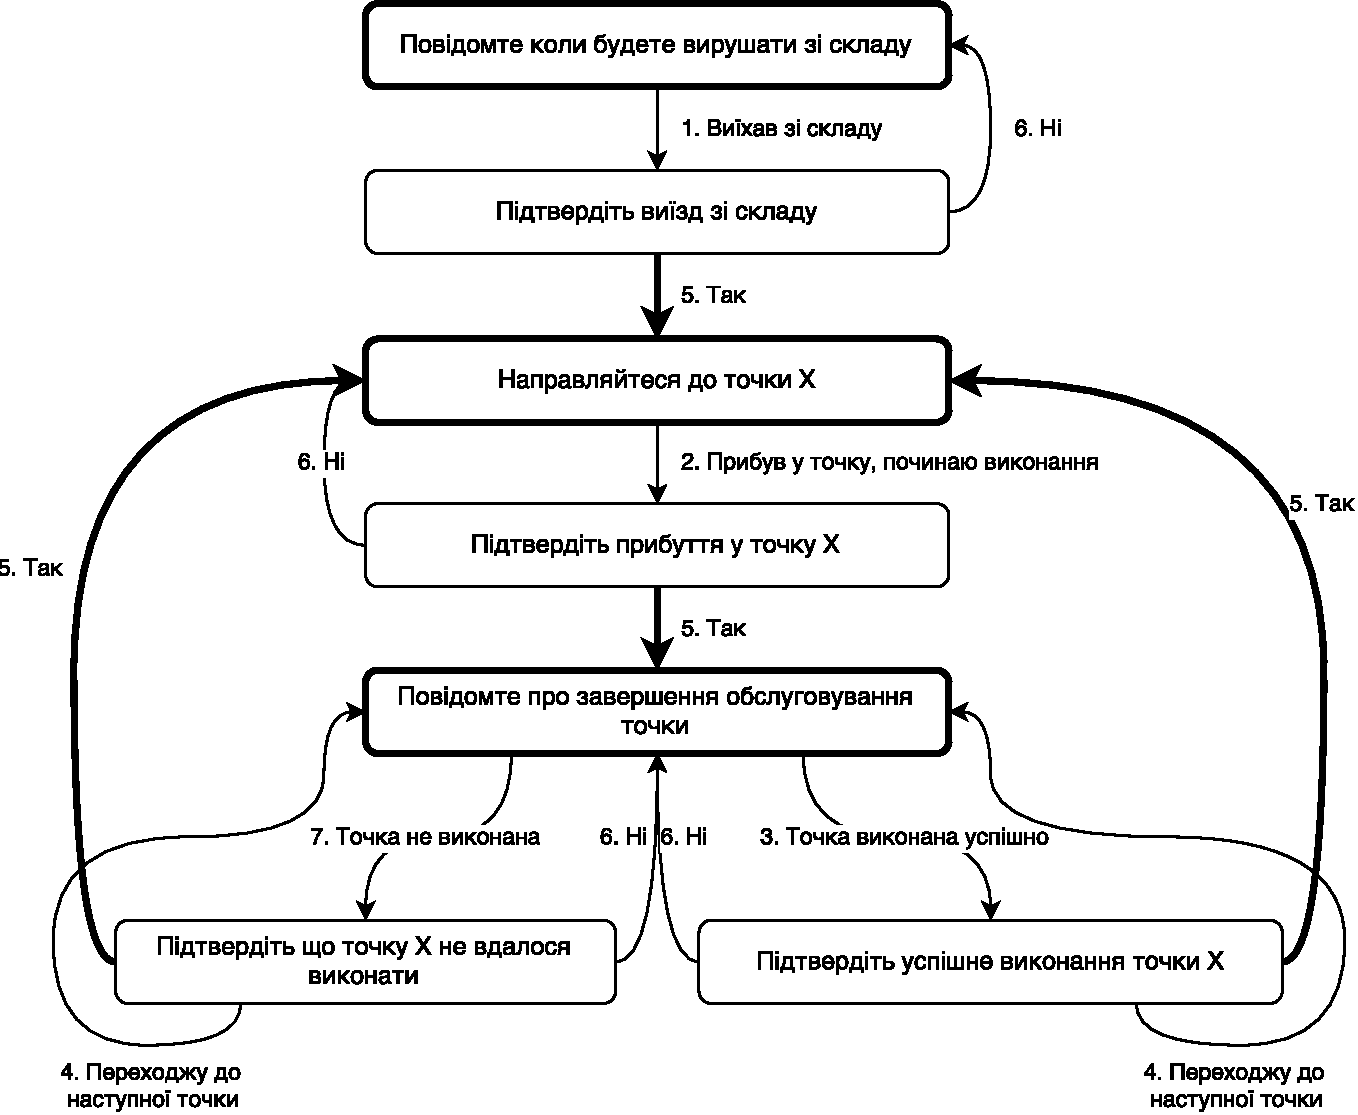
\includegraphics [width=.8\linewidth] {05_simple_negative_scenario_with_conformation}
	\caption{Варіант дерева сценаріїв з негативними інцидентами}
	\label{img:05_simple_negative_scenario_with_conformation}
\end{figure}

На рис. \ref{img:05_simple_negative_scenario_with_conformation} з’являється додатковий блок, пов’язаний з підтвердженням того, що точку Х не вдалося виконати, тобто дерево сценаріїв включає можливі негативні інциденти в моделі голосової взаємодії водія в системах диспетчерського контролю за рухом автотранспорту.

Також у моделі голосової взаємодії водія в системах диспетчерського контролю за рухом автотранспорту може бути запропонований один з варіантів дерева сценаріїв з негативними інцидентами та відбоєм (рис. \ref{img:06_simple_negative_scenario_with_rollback}). Для наведеного випадку з’являється блок у дереві сценаріїв, пов’язаний з підтвердженням неприбуття на точку Х. Тобто в дереві сценаріїв з’являється зв’язок з відбоєм виконання та обслуговування точки Х при моделюванні голосової взаємодії водія в системах диспетчерського контролю за рухом автотранспорту.

\begin{figure}
	\centering
	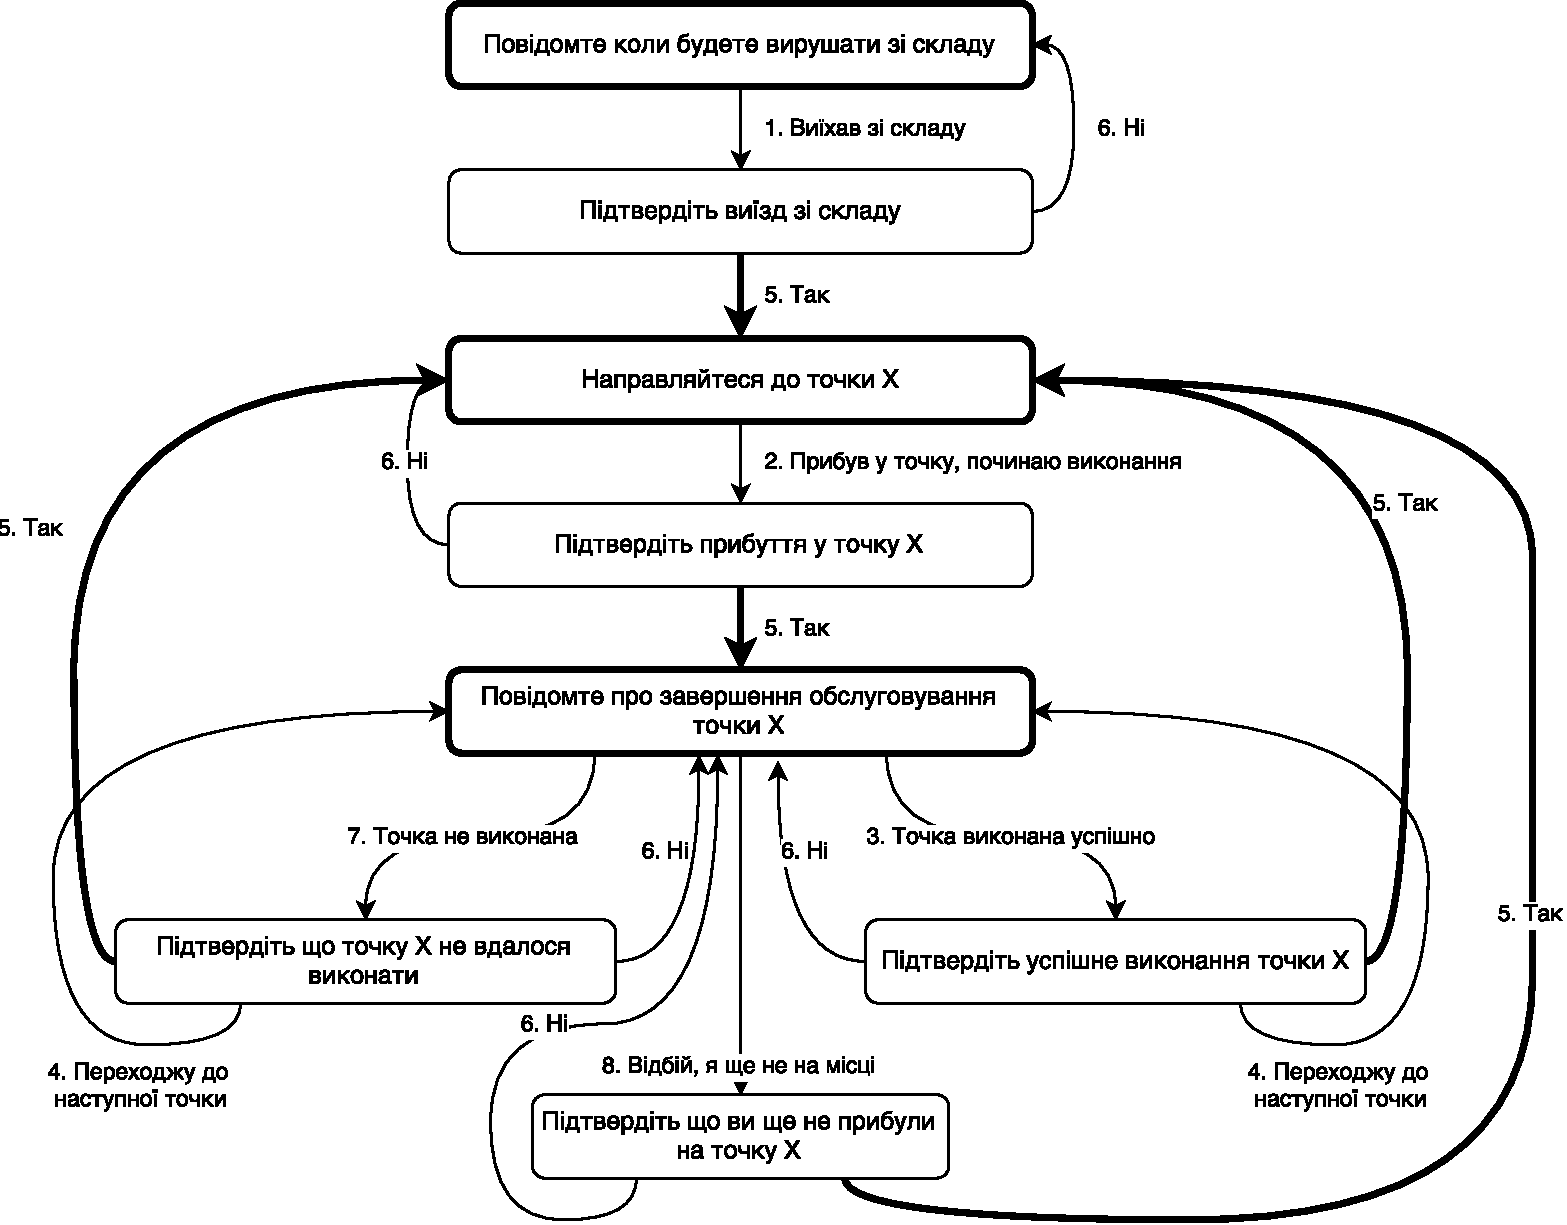
\includegraphics [width=.8\linewidth] {06_simple_negative_scenario_with_rollback}
	\caption{Варіант дерева сценаріїв з негативними інцидентами та відбоєм}
	\label{img:06_simple_negative_scenario_with_rollback}
\end{figure}

Приведені фрагменти дерева сценаріїв етапу «точка доставки» у вертикальному (рис. \ref{img:06_simple_negative_scenario_with_rollback}) розподілі включають виконання та обслуговування попередньої точки Y, поточної точки Х та наступної Z, що розташовані на відповідних дорогах.

Оскільки дерево стає занадто великим для зображення, для подальшої деталізації розбиваємо його на частини згідно до трьох основних етапів. Частина дерева сценаріїв етапу «точка доставки» у вертикальному розподілі приведена на рис. \ref{img:07_simple_point_scenario}.

На рис. \ref{img:08_complete_point_scenario} приведена одна з частин дерева сценаріїв етапу «точка доставки» з всіма негативними інцидентами при моделюванні голосової взаємодії водія в системах диспетчерського контролю за рухом автотранспорту.

\begin{figure}
	\centering
	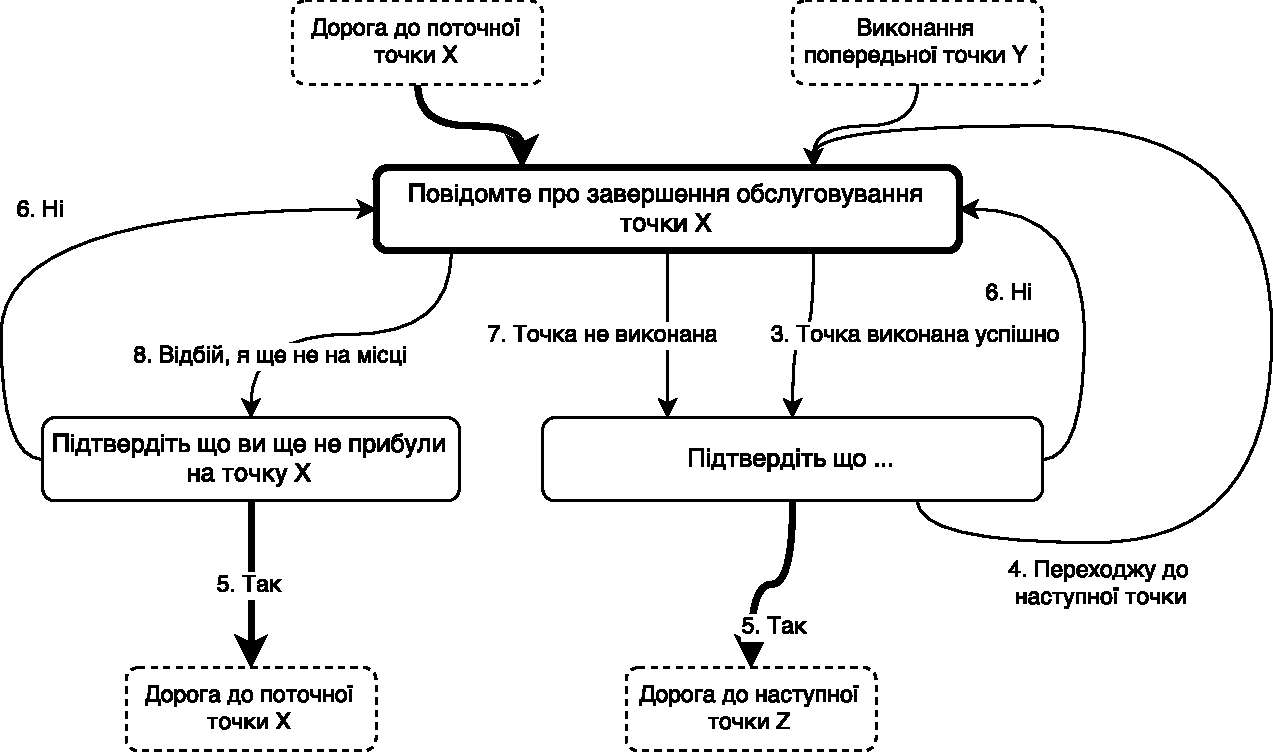
\includegraphics [width=.8\linewidth] {07_simple_point_scenario}
	\caption{Частина дерева сценаріїв етапу <<точка доставки>>}
	\label{img:07_simple_point_scenario}
\end{figure}

\begin{figure}
	\centering
	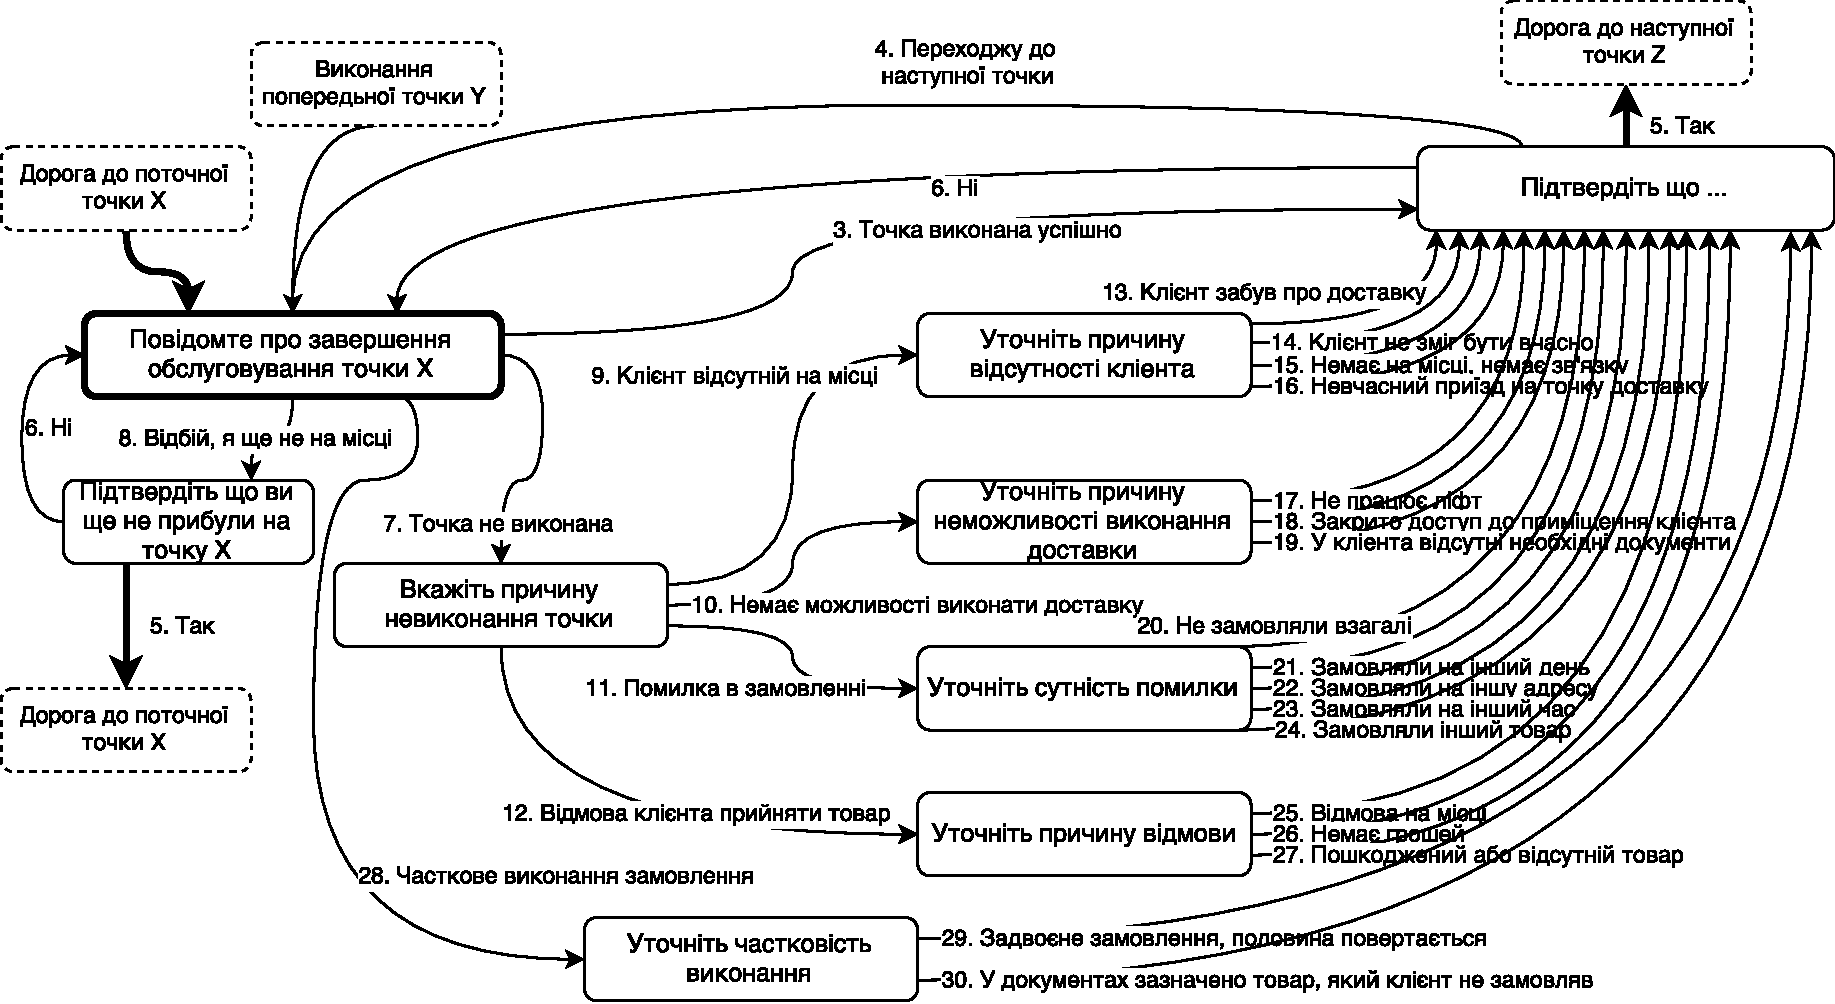
\includegraphics [width=.8\linewidth] {08_complete_point_scenario}
	\caption{Частина дерева сценаріїв етапу <<точка доставки>> з всіма негативними інцидентами}
	\label{img:08_complete_point_scenario}
\end{figure}

Приведена частина дерева сценаріїв етапу «точка доставки» (рис. \ref{img:08_complete_point_scenario}) включає блок невиконання точки Х з розширеним уточненням причин та блок часткового виконання з характеристиками такого виконання.

На етапі «дорога» – дерево сценаріїв для моделі голосової взаємодії водія в системах диспетчерського контролю за рухом автотранспорту має наступний вигляд (рис. \ref{img:11_complete_road_scenario}). У наведеній частині дерева сценаріїв етапу «дорога» враховані всі контексти з репрезентативної вибірки даних, що отримані у ведучих логістичних компаніях України. При цьому, у випадку невиконання етапу «дорога» пропонуються причини затримки чи неможливості виконання маршруту з наступними інструкціями диспетчера, а у випадку, коли з’являється можливість виконання маршруту до точки доставки Х існує відбій із діалогового режиму.

\begin{figure}
	\centering
	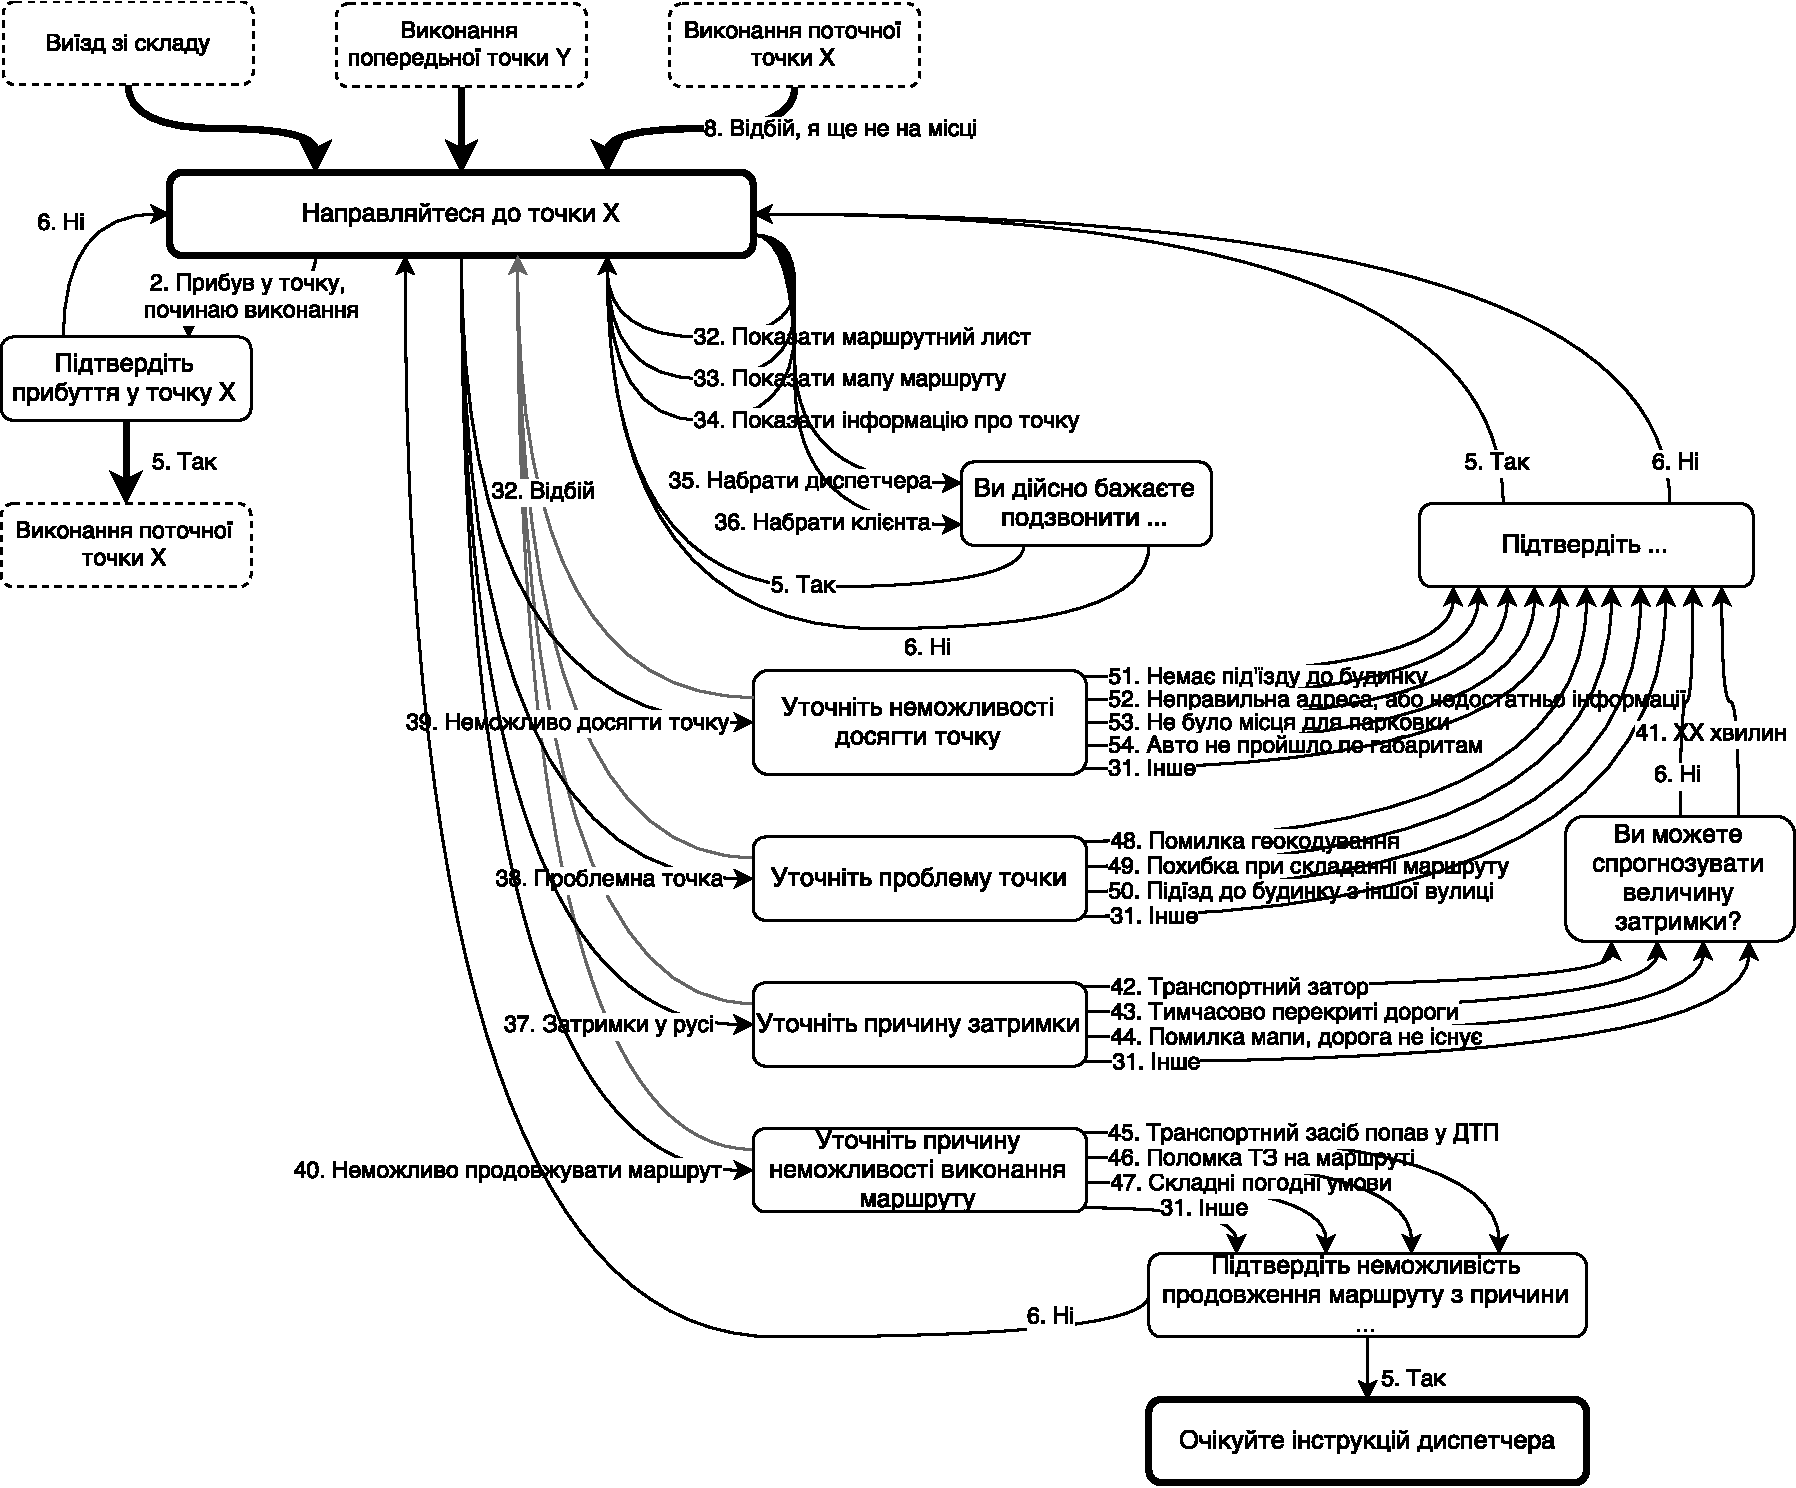
\includegraphics [width=.8\linewidth] {11_complete_road_scenario}
	\caption{Частина дерева сценаріїв етапу <<дорога>>}
	\label{img:11_complete_road_scenario}
\end{figure}

Для виконання етапу «склад» суб’єктом дистрибуції – водієм при його голосовій взаємодії в системі диспетчерського контролю за рухом автотранспорту побудовано дерево сценаріїв етапу «склад», частина якого приведена на рис. \ref{img:12_complete_depot_scenario}. В побудованому дереві сценаріїв етапу «склад» ураховані негативні причини затримки чи невиїзду зі складу з можливістю отримати подальші інструкції диспетчера для вирішення проблеми.

Повне дерево сценаріїв усіх етапів дистрибуції «склад – дорога – точка доставки» з вказівкою контекстів приведено на рис. \ref{img:14_complete_scenario_graph_contexts}. Повне дерево сценаріїв можна використати, щоб знайти і пронумерувати унікальні контексти (набори варіантів стимулів). Самі контексти або стани задають перелік дозволених стимулів, які може сприйняти система в знаходячись в цьому контексті.

\begin{figure}
	\centering
	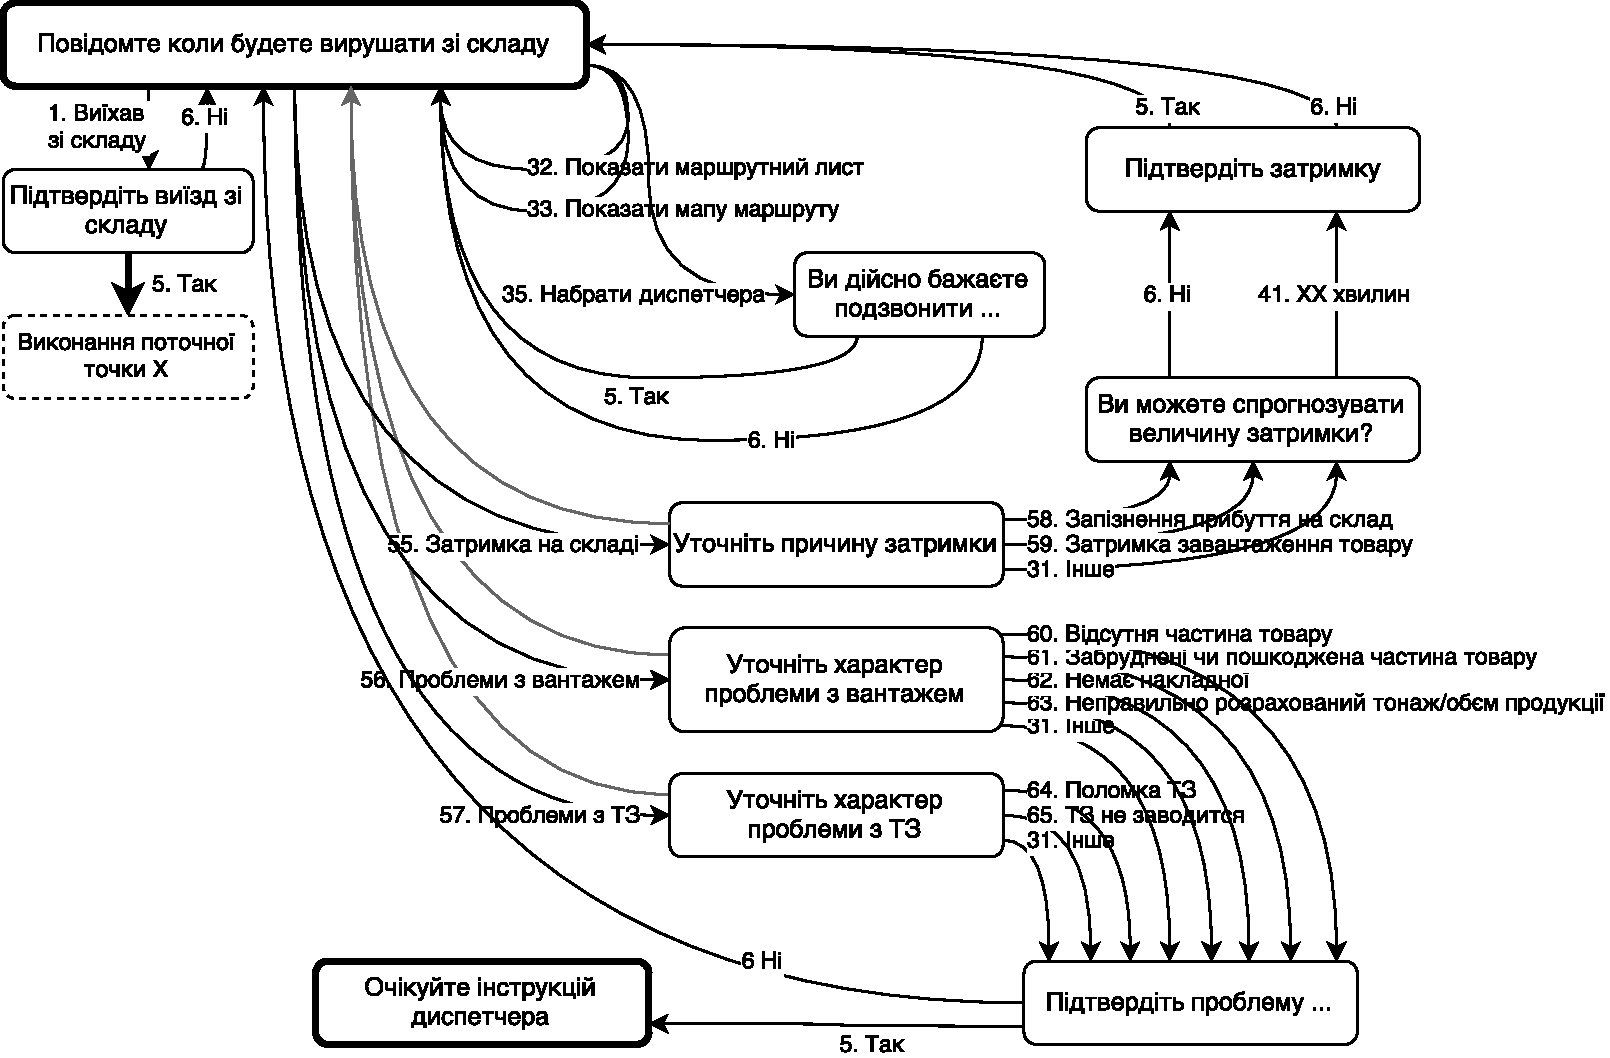
\includegraphics [width=.8\linewidth] {12_complete_depot_scenario}
	\caption{Частина дерева сценаріїв етапу <<склад>>}
	\label{img:12_complete_depot_scenario}
\end{figure}

\begin{figure}
	\centering
	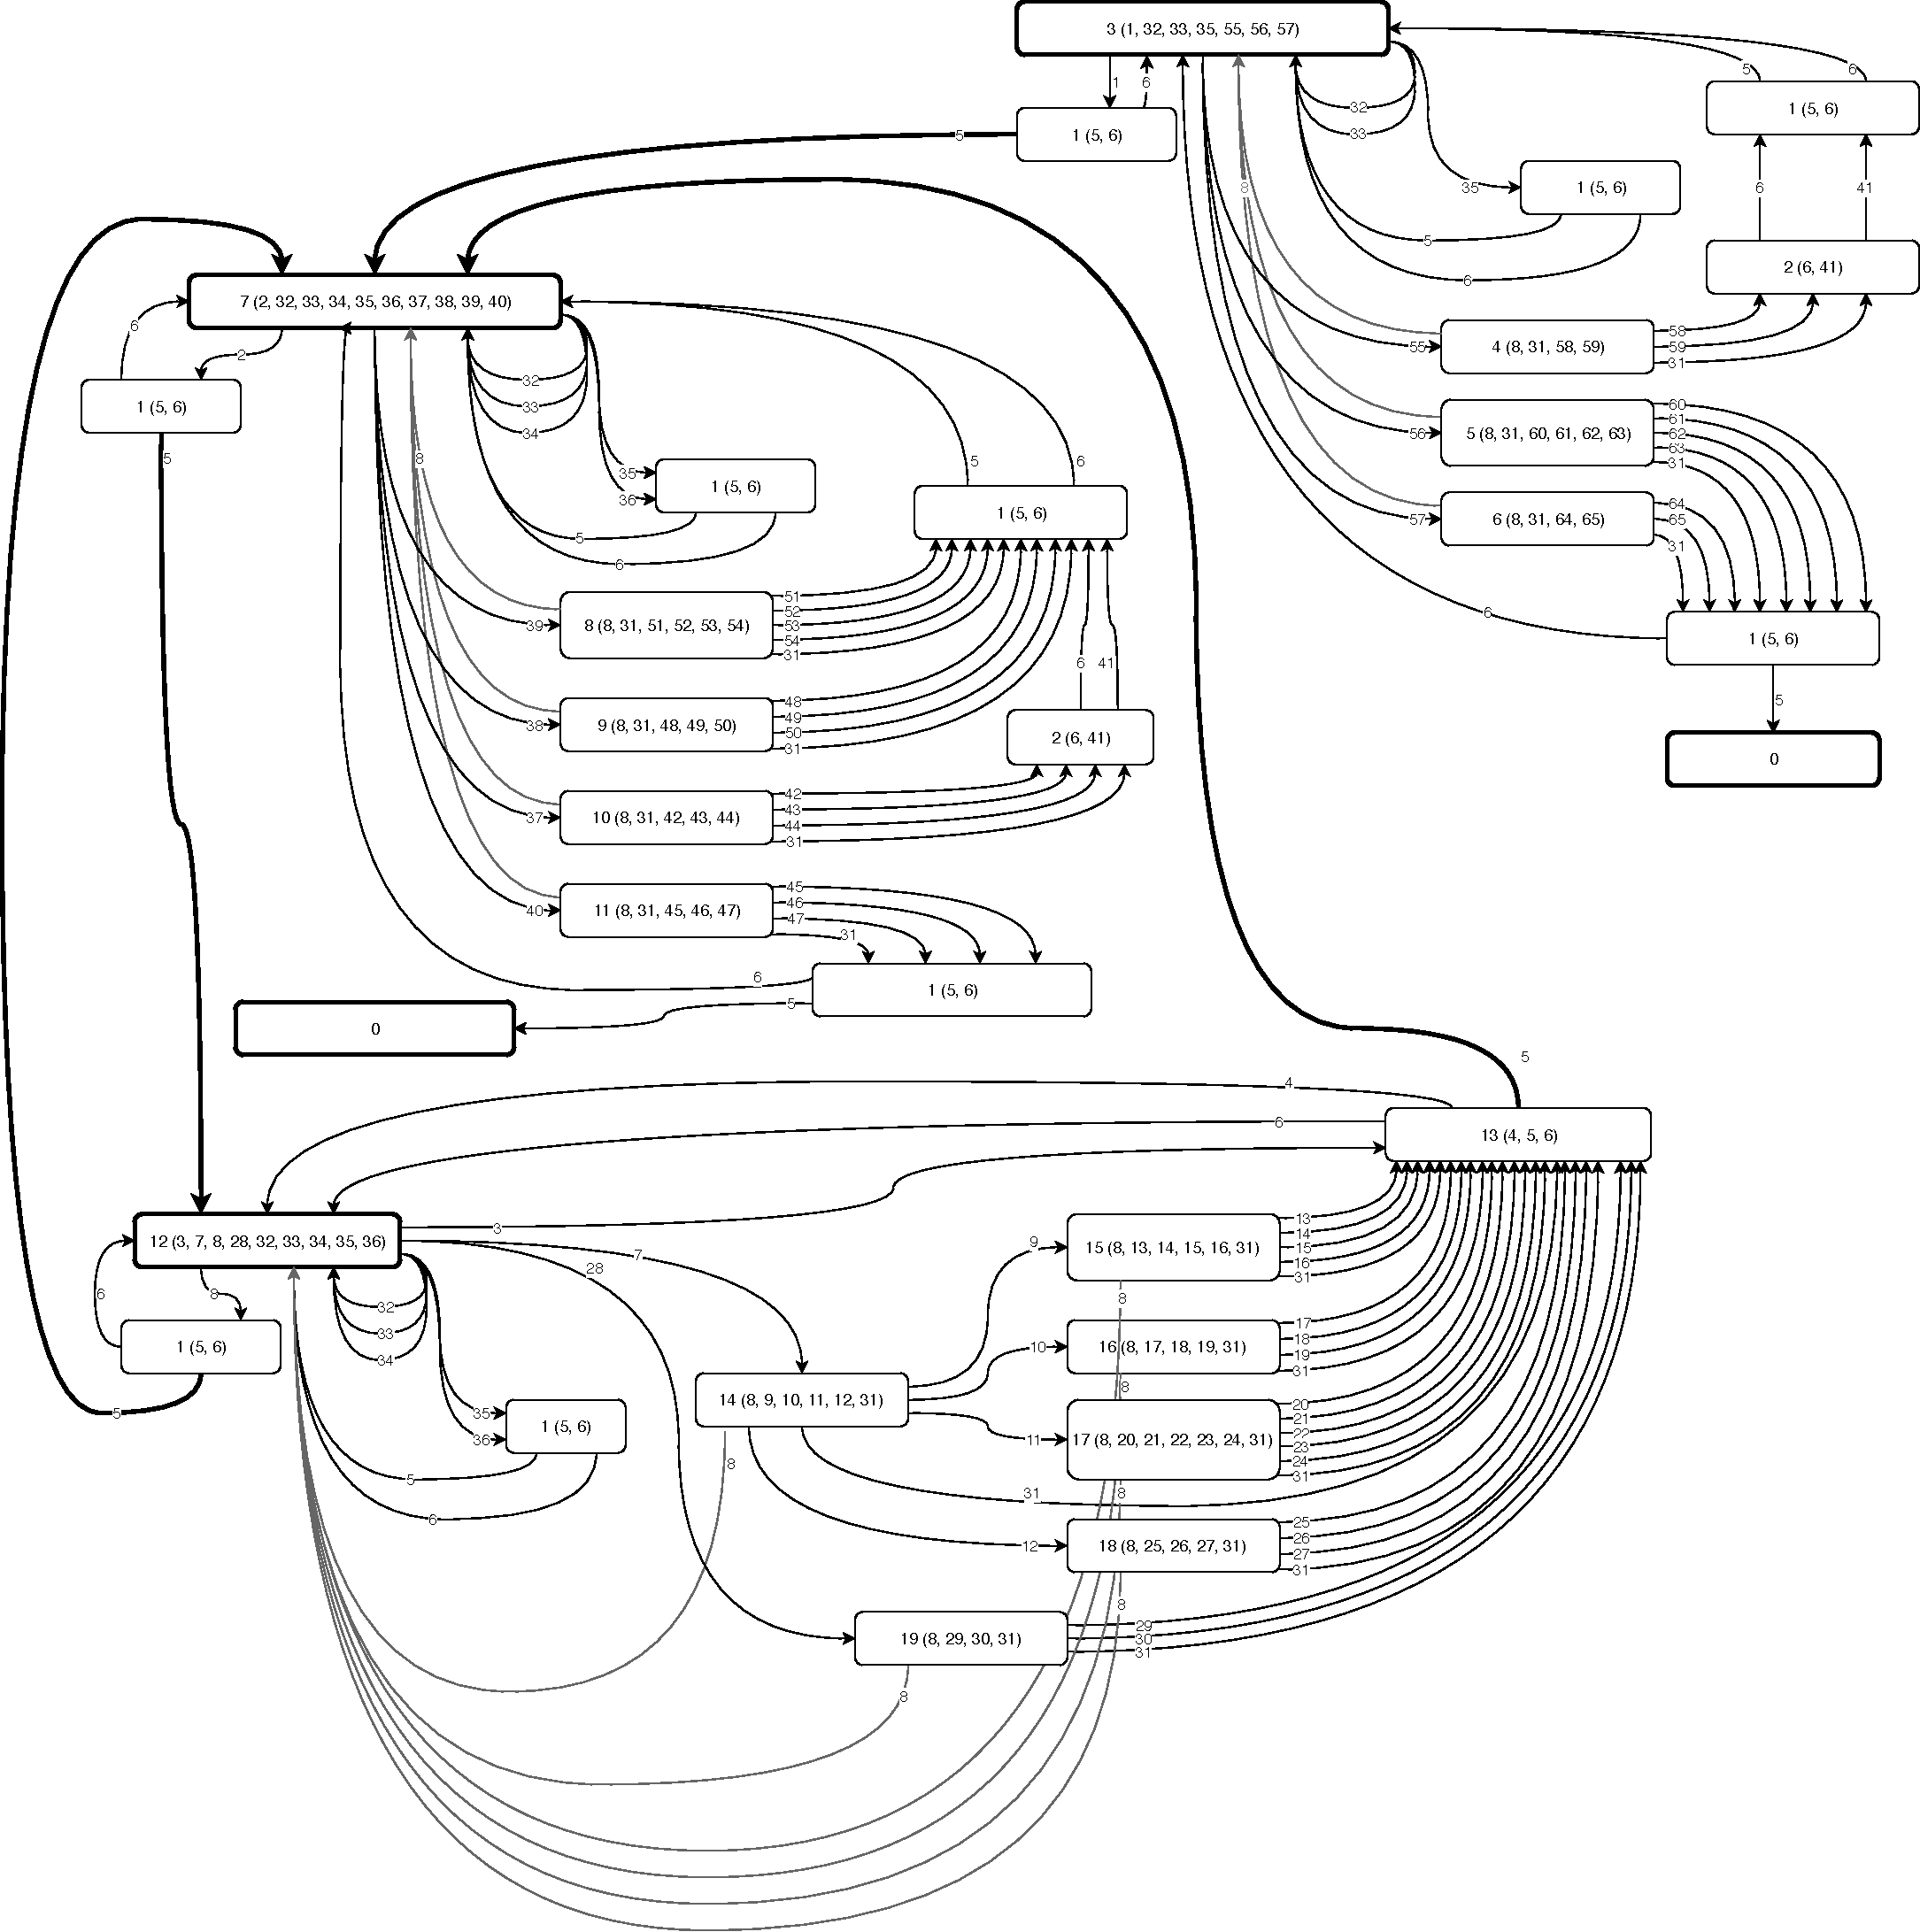
\includegraphics [width=.8\linewidth] {14_complete_scenario_graph_contexts}
	\caption{Повне дерево сценаріїв всіх етапів з указанням контекстів}
	\label{img:14_complete_scenario_graph_contexts}
\end{figure}

\section{Висновки}

У роботі запропоновано та розроблено модель голосової взаємодії водія в системах диспетчерського контролю за рухом автотранспорту. Рефлекторна модель розпізнання побудована за аналогією зі структурою умовного рефлексу, в якому виділяються афектори, центральний компонент та ефектори і поєднана з ідеєю використання дерева сценаріїв, оскільки сценарії також складаються із реакцій, і одиницею моделювання стає не лінгвістична особливість мовлення, а реакція (або команда), яка може бути врахована автоматизованою системою підрахунку маршрутів. У результаті запропоновано повне дерево сценаріїв усіх етапів дистрибуції «склад – дорога – точка доставки» з вказівкою контекстів і з включенням можливих реакцій в них, тобто на кожний позначений контекст існує реакція, що вказана в дужках на дереві сценаріїв.